\chapter{System Design}
\section{Design Approach}
\textbf{What are neural networks?}\\
An Artificial Neural Network (ANN) is an information processing paradigm that is inspired by the way biological nervous systems, such as the brain, process information. The key element of this paradigm is the novel structure of the information processing system. It is composed of a large number of highly interconnected processing elements (neurones) working in unison to solve specific problems. ANNs, like people, learn by example. An ANN is configured for a specific application, such as pattern recognition or data classification, through a learning process. Learning in biological systems involves adjustments to the synaptic connections that exist between the neurones.\\\\
\textbf{Why use neural networks?}\\
Neural networks, with their remarkable ability to derive meaning from complicated or imprecise data, can be used to extract patterns and detect trends that are too complex to be noticed by either humans or other computer techniques. A trained neural network can be thought of as an "expert" in the category of information it has been given to analyse. This expert can then be used to provide projections given new situations of interest and answer "what if" questions. Other advantages include:
\begin{itemize}
	\item \textbf{Adaptive learning:} An ability to learn how to do tasks based on the data given for training or initial experience.
	\item \textbf{Self-Organisation:} An ANN can create its own organisation or representation of the information it receives during learning time.
	\item \textbf{Real Time Operation:} ANN computations may be carried out in parallel, and special hardware devices are being designed and manufactured which take advantage of this capability.
	\item \textbf{Fault Tolerance via Redundant Information Coding:} Partial destruction of a network leads to the corresponding degradation of performance. However, some network capabilities may be retained even with major network damage.
\end{itemize}

Object Oriented design approach has been used for this project.
The datasets used in the CNN training consists of two large emotion datasets, namely the Toronto Face Database (TFD) with 4,178 images and the Facial Expression Recognition dataset (FER2013) containing 35,887 images, both with seven basic expressions: angry, disgust, fear, happy, sad, surprise and neutral.

Deep learning is a popular technique used in computer vision. I chose convolutional neural network (CNN) layers as building blocks to create my model architecture. CNNs are known to imitate how the human brain works when analysing visuals.

A typical architecture of a convolutional neural network will contain an input layer, some convolutional layers, some dense layers (aka. fully-connected layers), and an output layer as show in the figure below.

\begin{figure}[h]
	\centering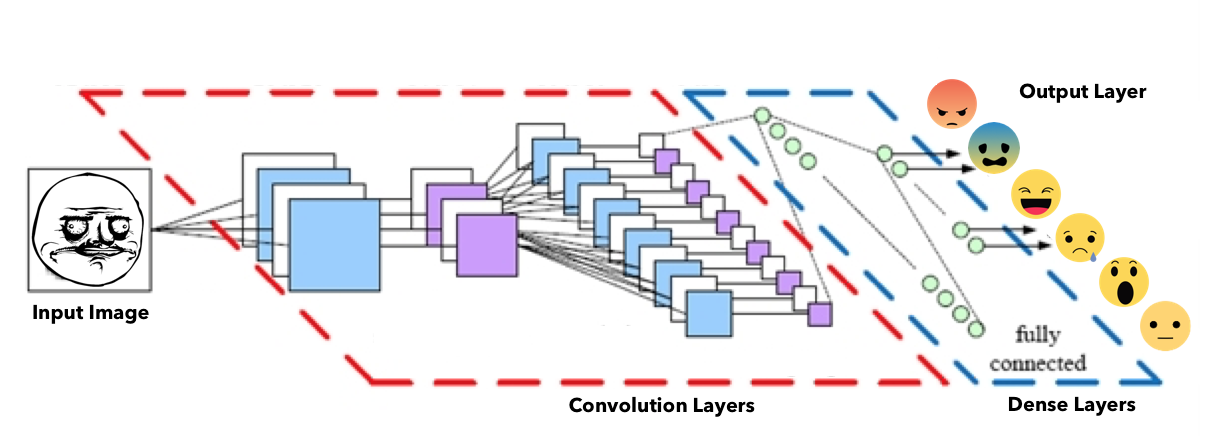
\includegraphics[scale=0.70]{images/problem_formulation.png}
	\caption{Facial Emotion Recognition CNN Architecture}
\end{figure}

\subsection{Input Layer}
\begin{itemize}
	\item The input layer has pre-determined, fixed dimensions, so the image must be pre-processed before it can be fed into the layer. I used OpenCV, a computer vision library, for face detection in the image. The haarcascade\_frontalface\_default.xml in OpenCV contains pre-trained filters and uses Adaboost to quickly find and crop the face.
	\item The cropped face is then converted into grayscale using cv2.cvtColor and resized to 48-by-48 pixels with cv2.resize. This step greatly reduces the dimensions compared to the original RGB format with three color dimensions (3, 48, 48). The pipeline ensures every image can be fed into the input layer as a (1, 48, 48) numpy array.
\end{itemize}

\subsection{Convolutional Layers}
\begin{itemize}
	\item \textbf{Numpy} array gets passed into the Convolution2D layer where I specify the number of filters as one of the hyper parameters. The set of filters(aka. kernel) are unique with randomly generated weights. Each filter, (3, 3) receptive field, slides across the original image with shared weights to create a feature map.
	\item \textbf{Convolution} generates feature maps that represent how pixel values are enhanced, for example, edge and pattern detection. In Figure 5, a feature map is created by applying filter 1 across the entire image. Other filters are applied one after another creating a set of feature maps.
	
	\begin{figure}[h]
		\centering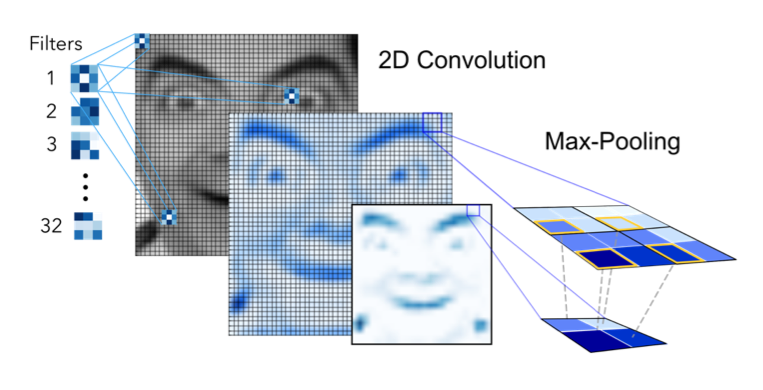
\includegraphics{images/conv_maxpool.png}
		\caption{Convolution and 1st max-pooling used in the network}
	\end{figure}

	\item \textbf{Pooling} is a dimension reduction technique usually applied after one or several convolutional layers. It is an important step when building CNNs as adding more convolutional layers can greatly affect computational time. I used a popular pooling method called MaxPooling2D that uses (2, 2) windows across the feature map only keeping the maximum pixel value. The pooled pixels form an image with dimentions reduced by 4.
\end{itemize}

\subsection{Dense Layers}
\begin{itemize}
	\item The dense layer (aka fully connected layers), is inspired by the way neurons transmit signals through the brain. It takes a large number of input features and transform features through layers connected with trainable weights.
	\item These weights are trained by forward propagation of training data then backward propagation of its errors. Back propagation starts from evaluating the difference between prediction and true value, and back calculates the weight adjustment needed to every layer before. We can control the training speed and the complexity of the architecture by tuning the hyper-parameters, such as learning rate and network density. As we feed in more data, the network is able to gradually make adjustments until errors are minimized.
	\item Essentially, the more layers/nodes we add to the network the better it can pick up signals. As good as it may sound, the model also becomes increasingly prone to over-fitting the training data. One method to prevent over-fitting and generalize on unseen data is to apply drop-out. Drop-out randomly selects a portion (usually less than 50\%) of nodes to set their weights to zero during training. This method can effectively control the model's sensitivity to noise during training while maintaining the necessary complexity of the architecture.
\end{itemize}

\subsection{Output Layer}
\begin{itemize}
	\item Instead of using sigmoid activation function, I used softmax at the output layer. This output presents itself as a probability for each emotion class.
	\item Therefore, the model is able to show the detail probability composition of the emotions in the face. As later on, you will see that it is not efficient to classify human facial expression as only a single emotion. Our expressions are usually much complex and contain a mix of emotions that could be used to accurately describe a particular expression.
\end{itemize}

\section{Detail Design}
\begin{figure}[h]
	\centering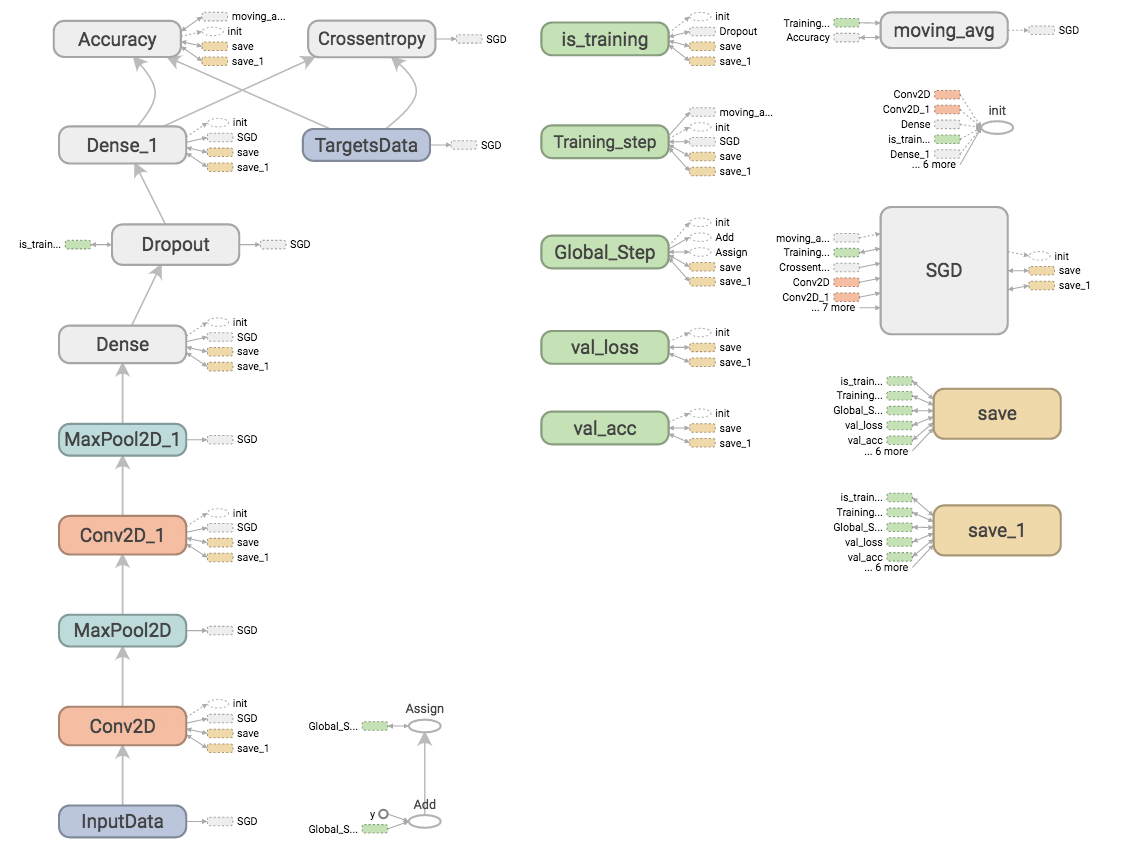
\includegraphics[scale=0.70]{images/graph.png}
	\caption{DNN Architecture}
\end{figure}

Neural networks, and deep networks in particular, are known for their need for large amounts of training data. Moreover, the choice of images used for training are responsible for a big part of the performance of the eventual model. This implies the need for a both high qualitative and quantitative dataset. For emotion recognition, several datasets are available for research, varying from a few hundred high resolution photos to tens of thousands smaller images. The three we will discuss are the Facial Expression Recognition Challenge (FERC-2013), Extended Cohn-Kanade (CK+) and Radboud Faces Database (RaFD)

The datasets differ mainly on quantity, quality, and ’cleanness’ of the images. The FERC-2013 set for example has about 32000 low resolution images, where the RaFD provides 8000 high resolution photos. Furthermore it can be noticed that the facial expressions in the CK+ and RaFD are posed (i.e. ’clean’), while the FERC-2013 set shows emotions ’in the wild’. This makes the pictures from the FERC-2013 set harder to interpret, but given the large size of the dataset, the diversity can be beneficial for the robustness of a model. 

We reason that, once trained upon the FERC-2013 set, images from ’clean’ datasets can easily be classified, but not vice versa. Hence for the three networks under consideration, training will be done using 9000 samples from the FER-2013 data (see figure 2) with another 1000 new samples for validation. Subsequently testing will be done with 1000 images from the RaFD set to get an indication of performance on clean high quality data. This latter set has an even distribution over all emotions.

\begin{figure}[h]
	\centering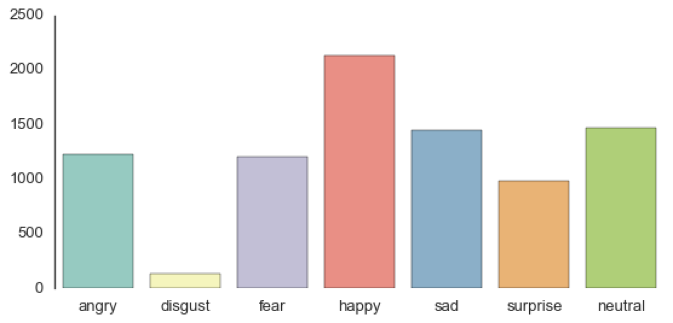
\includegraphics{images/fer2013.png}
	\caption{Number of images per emotion in the training set}
\end{figure}

Please note that non-frontal faces and pictures with the label contemptuous are taken out of the RaFD data, since these are not represented in the FERC-2013 training set. Furthermore, with use of the Haar Feature-Based Cascaded Classifier inside the OpenCV framework, all data is preprocessed. For every image, only the square part containing the face is taken, rescaled, and converted to an array with 48x48 grey-scale values.

\begin{figure}[h]
	\centering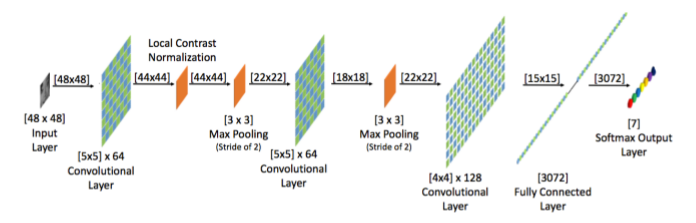
\includegraphics[scale=0.75]{images/network_architecture.png}
	\caption{Overview of the network architecture of the final model}
\end{figure}

\subsection{Networks}
The networks are programmed with use of the TFLearn library on top of TensorFlow, running on Python. This environment lowers the complexity of the code, since only the neuron layers have to be created, instead of every neuron. The program also provides real-time feedback on training progress and accuracy, and makes it easy to save and reuse the model after training. More details on this framework can be found in reference.

Since this research also aimed on recognizing 7 emotions using the FERC-2013 dataset, the architecture should be a good starting point for our research.

The original network starts with an input layer of 48 by 48, matching the size of the input data. This layer is followed by one convolutional layer, a local contrast normalization layer, and a maxpooling layer respectively. The network is finished with two more convolutional layers and one fully connected layer, connected to a softmax output layer. Dropout was applied to the fully connected layer and all layer contain ReLu units.

We therefore will train the network for 100 epochs in the final run, to make sure the accuracy converges to the optimum. In an attempt to improve the final model even more, the network will be trained on a larger set than the one described previously. Instead of 9000 pictures, training will be done with 20000 pictures from the FERC2013 dataset.

\section{User Interface Design}
\begin{figure}[h]
	\centering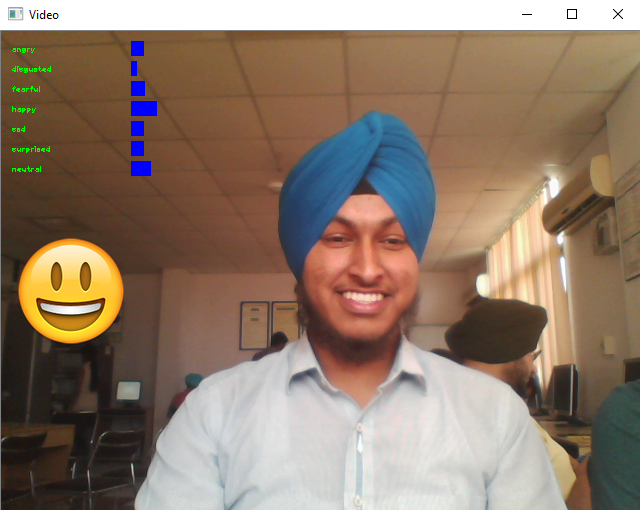
\includegraphics[scale=0.75]{images/ui.png}
	\caption{Live application with User Interface}
\end{figure}

Live emotion recognition through video is one of the most important key-points in human-machine interaction. To show the capabilities of the obtained network, an application is developed that can directly process web-cam footage through the final model.

With use of the aforementioned OpenCV face recognition program, the biggest appearing face from real-time video is tracked, extracted, and scaled to usable 48x48 input. This data is then fed to the input of the neural network model, which in its turn returns the values of the output layer. These values represent the likelihood that the each emotion is depicted by the user. The output with the highest value is assumed to be the current emotion of the user, and is depicted by an emotion on the left of the screen

Although it is hard to objectively assess, the live application shows promising performance. Though, it encounters problems when shadows are present on the face of the subject. All emotions are easily recognized when acted by the user, and when pointing the camera on the television, most emotions in the wild can be classified This once again emphasizes the power of using neural network based models for future applications in emotion recognition.

\section{Dataset Design}
IntraFace uses SIFT features for feature mapping and trains a descent method by a linear regression on training set in order to extract 49 points. We use these points to register faces to an average face in an affine transformation.

Finally, a fixed rectangle around the average face is considered as the face region.

Once the faces have been registered, the images are resized to 48x48 pixels for analysis. Even though many databases are composed of images with a much higher resolution testing suggested that decreasing this resolution does not greatly impact the accuracy, however vastly increases the speed of the network. To augment our data, we extract 5 crops of 40x40 from the four corners and the center of the image and utilize both of them and their horizontal flips for a total of 10 additional images.
\begin{figure}[h]
	\centering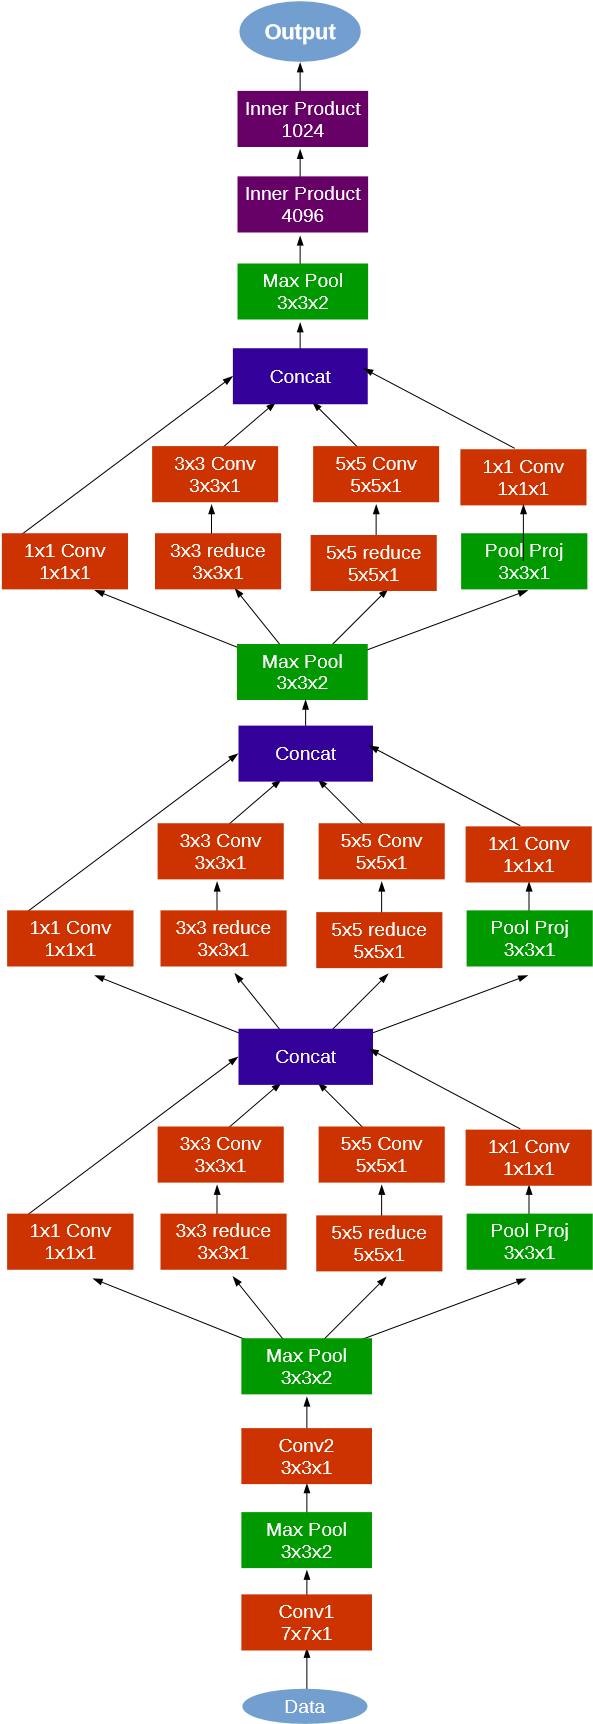
\includegraphics[scale=1.5]{images/dataset_design.png}
	\caption{Dataset Design Architecture}
\end{figure}

\section{Methodology}
\textbf{{\Large Feature Extraction}}\\
Different emotional states can be recognized using certain speech features which can be either prosody features or quality features. Some Prosody features which can be extracted directly; includes pitch, intensity and energy are the most widely used features in the emotion recognition domain. 